%\documentclass[a4paper,12pt,final,twoside]{scrartcl}
\setcounter{secnumdepth}{3}
\setcounter{tocdepth}{5}

\usepackage[utf8]{inputenc}
\usepackage[T1]{fontenc}
\linespread{1.4}
\usepackage{dsfont}
\usepackage{amsfonts}
\usepackage{amsmath}
\usepackage{amssymb}
\usepackage{amsthm}
\usepackage{mathtools}
\usepackage{mathbbol}
\usepackage{amsmath1}
\usepackage[ngerman]{babel}
\usepackage{bibgerm}
\usepackage[pdftex]{graphicx}
%\usepackage{mathpazo}
\usepackage{floatflt}
%%\usepackage{epsfig}
\usepackage{wrapfig}
\usepackage{graphicx}
\usepackage{tabularx}
\usepackage{caption} 
\usepackage{multicol} 
\usepackage{mathrsfs}
%\usepackage{pspicture}
%\usepackage{eepic}
%\usepackage{epic}
%\usepackage{trfsigns}

%\usepackage[ansinew]{inputenc}
\usepackage{longtable,array,dcolumn}
%\usepackage{ngerman}
\usepackage{epic}
\usepackage{rotate}
\usepackage{graphpap}
\usepackage{amssymb}
\usepackage[squaren]{SIunits}
\usepackage{curves}
\usepackage{float}
\usepackage{array}
\usepackage{enumerate}
\usepackage{marvosym}
\usepackage{slashed}%für feynmanslsash
\usepackage[breaklinks,pdfborder={0 0 0}]{hyperref}
\usepackage{ulem}	%angeblich funktioniert dann
\let\underbar\uline	%underbar in math auch bei greek letters
\usepackage{multirow}
%\usepackage{multicolumn}
\usepackage{enumitem}


\setlength{\parskip}{12pt}
\setlength{\parindent}{0mm}
%\newcommand{\grad}{\ensuremath{^{\circ}}
%\renewcommand{\figurename}{Abb.}		% mit usepackage caption2
%\renewcommand{\captionfont}{\small \itshape}	% mit usepackage caption2
%\setkomafont{caption}{\small \itshape}		%sollte mit caption im userpackage funktionieren
%\setkomafont{captionlabel}{\small , \itshape}	%sollte mit caption im userpackage funktionieren
\captionsetup{font = {small, sf}} %mit it anstelle von sf gibts kusiv

\date{2009-20-10}
\newcommand{\kreis}[1]{
 \qbezier(-#1,0)(-#1,#1)(0,#1)
  \qbezier(0,#1)(#1,#1)(#1,0)
  \qbezier(#1,0)(#1,-#1)(0,-#1)
  \qbezier(0,-#1)(-#1,-#1)(-#1,0)}
\newcommand{\s}{\ \big| \ }
\newcommand{\lo}{\left <}
\newcommand{\ro}{\ri >}
\newcommand{\g}{&=&}

\newcommand{\ham}{\mathcal H}
\newcommand{\hil}{\mathscr H}
\newcommand{\fok}{\mathscr F}
\newcommand{\wh}{\widehat}
%\newcommand{\left}{\left}
\newcommand{\ri}{\right}
\newcommand{\Sp}{\text{Sp}}
\newcommand{\babsatz}{\par \begingroup \leftskip=2cm}
\newcommand{\eabsatz}{\par\endgroup}

\newcommand{\D}{\text{\itshape D}}
\newcommand{\Lr}{\mathcal L }%\textit{L}}
\newcommand{\rot}{\text{rot}}
\newcommand{\divergenz}{\text{div}}
\newcommand{\grad}{\text{grad}}
\newcommand{\grat}{${}^{\circ}$}
%\newcommand{\tanh}{\text{tanh}} already defined

\newcommand{\RM}[1]{\text{\MakeUppercase{\romannumeral #1}}}
\newcommand{\dell}{\partial}
\renewcommand{\div}{\operatorname{div}}
\newcommand{\I}{\dot{\text{\i\!\i}}}
\newcommand{\e}{\mathrm{e}}
\newcommand{\ket}[1]{\mid\!\!\!\,\,{#1}\rangle}
\newcommand{\bra}[1]{\langle{#1}\!\!\!\,\,\mid}
\newcommand{\braket}[2]{\langle{#1}\!\!\!\,\,\mid\!\!\!\,\,{#2}\rangle}
\newcommand{\bracket}[3]{\langle{#1}\!\!\!\,\,\mid\!\!\!\,\,{#2}\!\!\!\,\,\mid\!\!\!\,\,{#3}\rangle}
\newcommand{\1}{\mathds{1}}
\newcommand{\EW}[1]{\langle\!\!\,\,#1\!\!\,\,\rangle}
\newcommand{\arrowbox}[1]{-\!\!\!\!\:\text{(#1)}\!\!\!\;\;\!\!\!\rightarrow}

\newcommand{\ketI}[1]{\ket{#1}_{\!\!\;\text{I}}}
\newcommand{\ketII}[1]{\ket{#1}_{\!\!\;\text{II}}}
\newcommand{\ketIII}[1]{\ket{#1}_{\!\!\;\text{III}}}
\newcommand{\braI}[1]{\,\!_{\text{I}\!\!\;}\bra{#1}}
\newcommand{\braII}[1]{\,\!_{\text{II}\!\!\;}\bra{#1}}
\newcommand{\braketI}[2]{\,_{\text{I}\!\!\;}\braket{#1}{#2}_{\!\!\;\text{I}}\,}
\newcommand{\braketII}[2]{\,_{\text{II}\!\!\;}\braket{#1}{#2}_{\!\!\;\text{II}}\,}
\newcommand{\braketIII}[2]{\,_{\text{III}\!\!\;}\braket{#1}{#2}_{\!\!\;\text{III}}\,}
\newcommand{\bracketI}[3]{\,_{\text{I}\!\!\;}\bracket{#1}{#2}{#3}_{\!\!\;\text{I}}\,}
\newcommand{\bracketII}[3]{\,_{\text{II}\!\!\;}\bracket{#1}{#2}{#3}_{\!\!\;\text{II}}\,}


\newcommand{\up}{\ket{\uparrow}}
\newcommand{\updg}{\bra{\uparrow}}
\newcommand{\down}{\ket{\downarrow}}
\newcommand{\downdg}{\bra{\downarrow}}
\newcommand{\upup}{\ket{\uparrow\uparrow}}
\newcommand{\updown}{\ket{\uparrow\downarrow}}
\newcommand{\downup}{\ket{\downarrow\uparrow}}
\newcommand{\downdown}{\ket{\downarrow\downarrow}}

\newenvironment{itemize1}{\begin{itemize}[leftmargin=5mm,itemsep=-1ex,topsep=-1ex]}{\end{itemize}}

%\usepackage[left=2cm,right=2cm,top=1cm,bottom=1cm,includeheadfoot]{geometry}

\usepackage{fancyhdr}
\pagestyle{fancy}{\fancyhf{}
\fancyhead[LO,RE]{\footnotesize \rightmark}
\fancyfoot[C]{\footnotesize -$\,$\thepage$\;$-}
\renewcommand{\headrulewidth}{0.4pt}
\renewcommand{\footrulewidth}{0pt}}

\fancypagestyle{plain}{\fancyhf{}
\renewcommand{\headrulewidth}{0.4pt}
\fancyfoot[C]{\footnotesize -$\,$\thepage$\,$-}}

\usepackage{titlesec}
\titleformat{\section}[display]{\sffamily\bfseries\Huge\center}{Kapitel \thetitle:}{1ex}{}{}
\newcommand{\kapitel}[2]{$\;$\vspace{-1.5cm} \section[#1]{#2} \rule{17cm}{0.4pt}\vspace{3cm}}
\titleformat{\paragraph}[hang]{\sffamily\bfseries}{\thetitle:}{0ex}{\vspace{-0.15cm}}{\vspace{0.5cm}}

\title{ \vspace{1.5cm}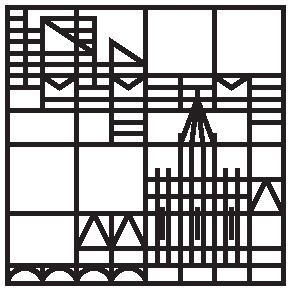
\includegraphics[width=5cm]{logo}
\\ \Large Universität Konstanz  \\ \vspace{4ex} \huge 
Skript zur Vorlesung\\ Höhere Quantentheorie und Elektrodynamik
\\ \vspace{4ex} \Large Prof. Dr. Wolfgang Belzig 
\\ Version vom 30. Juli 2012 \\ \vspace{4.5cm}
\normalsize Ursprünglichen Mitschrift von Birte Heinze im WS 09/10 \\ Ausführliche Überarbeitung von Tobias Lohse im WS 11/12 \vspace{-10cm}}
\author{}
\date{}
%\begin{document}

\subsection{Quantendynamik mit Propagatoren}
Im folgenden Abschnitt soll auf die Beschreibung der Dynamik quantenmechanischer Systeme mittels sogenannter Propagatoren eingegangen werden, welche schließlich auf die Pfadintegralformilierung der Quantenmechanik nach Feynman führt. 

\subsubsection{Propagatoren und die Greensche Funktion der Schrödingergleichung}
Wir wollen uns im folgenden mit der allgemeinen Lösung der Schrödingergleichung (\ref{SGL}) für einen zeitunanbhängigen Hamiltonoperator $\hat{\ham}$ im Ortsraum beschäftigen. 

Die Basis des Ortsraum besteht aus den Zuständen $\ket{x}$ mit $x\in\mathbb{R}$, ist also unendlich dimensional. Die Orthonormalität der Ortszustände wird dann mit der Deltafunktion notiert: $\braket{x}{x'}=\delta(x-x')$. Der Ket-Vektor $\ket{\psi}$ kann im Ortsraum geschrieben werden als Wellenfunktion: $\braket{x}{\psi(t)}=\psi(x,t)$. Die Lösung der Schrödingergleichung für einen zeitunabhängigen Hamiltonoperator ergibt sich, wie wir bereits gezeigt haben zu: 
\begin{eqnarray*} 
	\ket{\psi(t)} &=& \e^{-\frac{\I}{\hbar}\cdot \hat{\ham}\cdot(t-t')}\; \ket{\psi(t')}
\end{eqnarray*} 
Wenn wir in diese Gleichung eine $\1=\int \mathrm{d}x\;\ket{x}\bra{x}$ einfügen und beide Seiten von links mit $\bra{x}$ multiplizieren, so ergibt sich:
\begin{eqnarray}
	\braket{x}{\psi(t)} &=& \int\mathrm{d}x'\; \underbrace{\bracket{x}{\e^{-\frac{\I}{\hbar}\cdot\hat{\ham}\cdot(t-t')}}{x'}}_{=:\;K(x,t,x',t')} \cdot \braket{x'}{\psi(t)} \nonumber
	\\
	\Leftrightarrow\qquad \psi(x,t) &=& \int\mathrm{d}x'\; K(x,t,x't') \cdot\psi(x',t') \label{PropagatorDynamik}
\end{eqnarray}
Die Funktion $K(x,t,x',t')$ wird dabei als {\bf Propagator} bezeichnet. Die Bestimmung des Propagators ist somit äquivalent zur Lösung der zeitabhängigen Schrödingergleichung. Der Propagator beschreibt die Amplitude am Ort $x$ zur Zeit $t$, die von der Ausgangsamplitude bei $x'$ zur Zeit $t'$ verursacht wird. Der Endzustand ergibt sich also als Superposition der Anfangszustände mit Amplitudengewichtung $K(x,t,x',t')$. Der Propagator selbst erfüllt die Schrödingergleichung:
\begin{eqnarray*} 
	\I\hbar\cdot\dell_t\;K(x,t,x',t') = \hat{\ham}\;K(x,t,x',t') &\quad& \text{mit Anfangsbedingung: } K(x,t,x',t) = \delta(x-x')
\end{eqnarray*} 
Der Propagator hat somit eine gewisse Ähnlichkeit mit einer Greenschen Funktion. Und tatsächlich können wir mit seiner Hilfe leicht eine {\bf retardierte Greensche Funktion} $G_R(x,t,x',t')$ und eine {\bf avancierte Greensche Funktion} $G_A(x,t,x',t')$ der Schrödingergleichung einführen: 
\begin{eqnarray*}
	G_R(x,t,x't') = -\frac{\I}{\hbar}\cdot\Theta(t-t')\cdot K(x,t,x',t')
	\\
	G_A(x,t,x't') = \frac{\I}{\hbar}\cdot\Theta(t'-t)\cdot K(x,t,x',t')
\end{eqnarray*}
Die unterschiedlichen Theta-Funktionen sorgen dafür, dass die retardierte Greensche Funktion nur für kausale Zusammenhänge ungleich 0 ist und die avancierte nur für antikausale. In der Physik wird Kausalität dabei verstanden als zeitliche Abfolge von Zusammenhängen, deren Propagation eindeutig positiv bestimmt ist. 

Wenn wir die retardierte oder avancierte Greensche Funktion in die Schrödingergelichung einsetzten, lässt sich zeigen, dass es sich bei den von uns definierten Funktionen tatsächlich um Greensche Funktionen handelt: 
\begin{eqnarray*}
	\I\hbar\cdot\partial_t\; G_{R/A}(x,t,x',t') &=& \I\hbar \frac{\mp\I}{\hbar}\Big(K(x,t,x',t')\cdot\underbrace{\partial_t\;\Theta(\pm t\mp t')}_{=\;\delta(\pm t\mp t')} + \Theta(\pm t\mp t')\cdot\underbrace{\partial_t\; K(x,t;x',t')}_{= \hat{\ham}\;K(x,t,x',t')/\I\hbar}\Big)
	\\
	&=& \pm\Big(\underbrace{K(x,t,x',t)}_{=\;\delta(x-x')}\cdot\delta(t-t')\pm\hat{\ham}\;\underbrace{\frac{\mp\I}{\hbar}\cdot\Theta(\pm t\mp t')\cdot K(x,t,x',t')}_{=\;G_{R/A}(x,t,x',t')}\Big) 
	\\\;\\
	\Leftrightarrow\quad \big(\I\hbar\partial_t-\hat{\ham}\big)\; G_{R/A}(&&\!\!\!\!\!\!\!\!\!\!\!\!\!\!x,t,x',t') \;\;=\;\; \delta(x-x')\cdot\delta(t-t') 
\end{eqnarray*}
Wegen der Zeitumkehrinvarianz der Schrödingergleichung ist diese jedoch nicht hinreichend um die Greensche Funktion zu definieren, da sie keine Unterscheidung zwischen retardierter und avancierter Greenscher Funktion zulässt. 

Da die Greensche Funktion eine inhomogenen Differentialgleichungung erfüllt, ist sie im Fourierraum sehr leicht lösbar und ist somit bei der allgemeinen Lösung von Problemen hilfreich sein. 


\subsubsection{Greensche Funktion eines freien Teilchens}

Im folgenden wollen wir die Verwendung und Bestimmung der Greenschen Funktion am Beispiel eines freien Teilchens mit dem Hamiltonoperaotr $\hat{\ham}=-\triangle/2m$ erläutern. 

Die Fouriertransformierte der Greenschen Funktion $\tilde{G}(\omega,k)$ lässt sich leicht bestimmen und ist gegeben durch: 
\begin{eqnarray*}
	\widetilde{G}(\omega,k) \;\;=\;\; \frac{2m}{\omega-\hbar^2k^2} &=& \frac{1/\hbar}{\omega-\omega(k)} \quad\qquad\text{mit: } \omega(k) = \frac{\hbar k^2}{2 m} 
\end{eqnarray*}
Die Greensche Funktion ist dann bestimmt durch die Rücktransformation, welche sich als folgendes Integral schreiben lässt: 
\begin{eqnarray*}
	G(x,t,0,0) &=& \int\frac{\mathrm{d}\omega}{2\pi}\int\frac{\mathrm{d}k}{2\pi}\;\e^{\;\I(kx-\omega t)}\cdot \widetilde{G}(\omega,k)
\end{eqnarray*}
Allerdings besteht das Problem, dass die Fouriertransformierte Greensche Funktion $\tilde{G}$ singulär für $\omega(k)=\omega$ ist, sodass die Kausalität in diesem Fall unklar ist. Dies können wir lösen, indem wir die Frequenz $\omega$ um einen imaginären  Parameter verschieben und dann diesen Parameter gegen Null gehen lassen. 
\begin{eqnarray*} 
	\widetilde{G}_{R/A}(\omega,k) = \lim_{\delta\to0}\;\widetilde{G}(\omega\pm\I\delta,k)
\end{eqnarray*} 
Wir wollen uns zunächst mit dem Integral über $\mathrm{d}\omega$ für die Greensche Funktion beschäftigen: 
\begin{eqnarray*}
	\tilde{G}_{R/A}(t,k) &=& \lim_{\delta\to0}\;\;\frac{1}{\hbar}\cdot \int_{-\infty}^{+\infty}\!\!\!\mathrm{d}\omega\;\underbrace{\frac{\e^{-\I\omega t}/2\pi}{\omega-(\omega(k)\mp\I\delta)}}_{:=\;g_{R/A}(\omega)}
\end{eqnarray*}
Zur Berechnung dieses Integral können wir den {\bf Residuensatz} verwenden: 
\begin{eqnarray*}
	\oint_{\gamma}\mathrm{d}s\;f = 2\pi\I\cdot\sum_n\mathrm{ind}_{z_n}\cdot\text{Res}_f(z_n) \qquad\text{Pol erster Ordnung: } \text{Res}_f(z_0)=\lim_{z\to z_0}\;(z-z_0)\cdot f(z)
\end{eqnarray*}
Dabei sind $z_n$ die Polstellen der Funktion $f$ und $\mathrm{ind}_{z_n}$ die Windungszahlen der Polstelle. Wir wandeln das Integral dazu in eine Kurvenintegral in der komplexen Ebene von $\omega=|\omega|\cdot\e^{\;\I\varphi}$ um und lassen dann $|\omega|$ gegen unendlich gehen. Die folgende Skizze soll dies verdeutlichen: 
\begin{figure}[h!]\centering
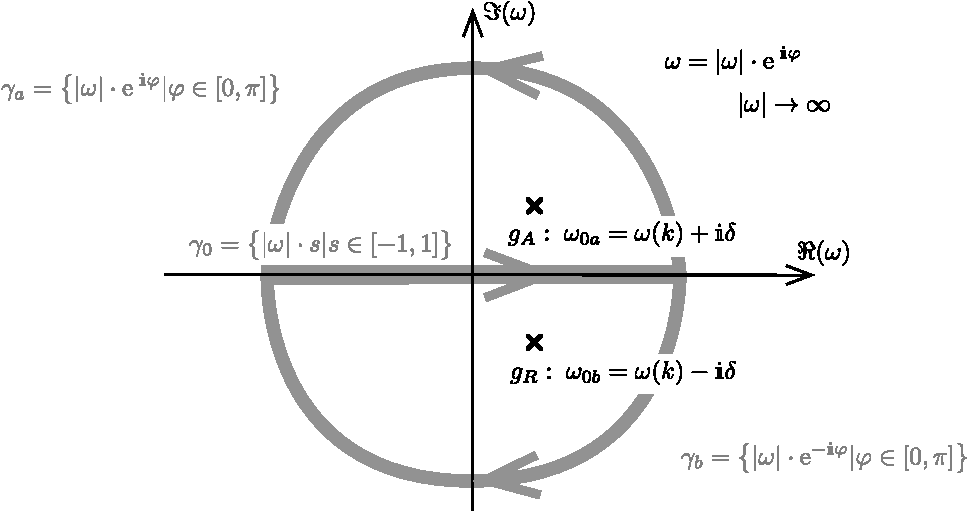
\includegraphics[scale=1]{Figs/komplexeebene}
\end{figure}

Wir erweitern den Integrationsweg $\gamma_0$ also um den oberen Integrationsweg $\gamma_a$ beziehungsweise den unteren Integrationsweg $\gamma_b$, um ein geschlossenes Kurvenitegral zu erhalten. Dies ist möglich, sofern für $|\omega|\to\infty$ dieses zusätzliche Kurvenintegral verschwindet. Ob das Integral über $\gamma_a$ beziehungsweise $\gamma_b$ verschwindet hängt dabei davon ab, ob die Zeit negativ oder positiv ist. Es lässt sich zeigen, dass gilt: 
\begin{eqnarray*}
	t>0:&\;&\int_{\gamma_a}\!\!\!\mathrm{d}s\; g_{R/A}=\int_0^{\pi}\!\!\!\mathrm{d}\varphi\;g_{R/A}\big(|\omega|\cdot\e^{\;\I\varphi}\big)\cdot|\omega|\;\underset{|\omega|\to\infty}{\to}\;\infty \qquad\land\qquad \int_{\gamma_b}\!\!\!\mathrm{d}s\; g_{R/A}\;\underset{|\omega|\to\infty}{\to}\;0
	\\\;\\
	t<0:&\;&\int_{\gamma_a}\!\!\!\mathrm{d}s\; g_{R/A}\;\underset{|\omega|\to\infty}{\to}\;0 \qquad\land\qquad \int_{\gamma_b}\!\!\!\mathrm{d}s\; g_{R/A}=\int_0^{\pi}\!\!\!\mathrm{d}\varphi\;g_{R/A}\big(|\omega|\cdot\e^{-\I\varphi}\big)\cdot|\omega|\;\underset{|\omega|\to\infty}{\to}\;\infty
\end{eqnarray*}
Wir können somit für $t>0$ den geschlossenen Integrationsweg $\gamma_0+\gamma_b$ wählen und für $t<0$ den geschlossenen Integrationsweg $\gamma_0+\gamma_a$. Wir müssen nun noch das Residuum für die beiden Integrationswege an den Polstellen der Funktionen $g_{R/A}$ berechnen. Dabei hat $g_R$ eine Polstelle bei $\omega_{0b}=\omega(k)-\I\delta$, die auf Weg $\gamma_0+\gamma_a$ nicht umlaufen wird und auf Weg $\gamma_0+\gamma_b$ mit Windungszahl $\mathrm{ind}_{\omega_0}=-1$ umlaufen wird. $g_A$ hat eine Polstelle bei $\omega_0=\omega(k)+\I\delta$, die auf Weg $\gamma_0+\gamma_a$ mit Windungszahl $\mathrm{ind}_{\omega_{0a}}=1$ umlaufen wird und auf Weg $\gamma_0+\gamma_b$ nicht umlaufen wird. Wir sehen somit, dass die Kausalität beziehungsweise Antikausalität für die retardierte undavancierte Greensche Funktion gewährlesitet ist. Es ergibt sich dann $\tilde{G}_{R/A}(t,k)$ zu: 
\begin{eqnarray*}
	\oint_{\gamma_0+\gamma_a}^{(t<0)}\!\!\!\!\!\!\!\!\!\mathrm{d}s\;g_A = 2\pi\I\cdot\text{Res}_{g_A}(\omega_{0a})= \lim_{\omega\to\omega_{0a}}\;\I\cdot\e^{-\I\omega t}\;=\;\I\cdot\e^{-\I(\omega(k)+\I\delta)t}\;\land\; \oint_{\gamma_0+\gamma_b}^{(t>0)}\!\!\!\!\!\!\!\!\!\mathrm{d}s\;g_R = -\I\cdot\e^{-\I(\omega(k)-\I\delta)t}
	\\
	\land\;\oint_{\gamma_0+\gamma_b}^{(t>0)}\!\!\!\!\!\!\!\!\!\mathrm{d}s\;g_A = \oint_{\gamma_0+\gamma_a}^{(t<0)}\!\!\!\!\!\!\!\!\!\mathrm{d}s\;g_R = 0 \qquad\Rightarrow\qquad\qquad \tilde{G}_{R/A}(t,k) = \mp\frac{\I}{\hbar}\cdot\Theta(\pm t)\cdot \e^{-\I\omega(k) t} \qquad\qquad
\end{eqnarray*}
Es bleibt noch das Integral über $\mathrm{d}k$ zu bestimmen. Dieses hat nun folgende Form: 
\begin{eqnarray*}
	G_{R/A}(t,x) &=& \mp \frac{\I}{\hbar}\cdot\Theta(\pm t)\cdot\int_{-\infty}^{+\infty}\frac{\mathrm{d}k}{2\pi}\; \e^{\I(kx-\omega(k)t)} 
\end{eqnarray*}
Der Exponent der e-Funktion im Integral kann dabei so umgeformt werden, dass sich ein Fresnelintegral ergibt, welches sich leicht lösen lässt: 
\begin{eqnarray} 
	&&\!\!\!\! \I\cdot\big(kx-\omega(k)t\big) = \I\cdot\Big(kx-\frac{\hbar k^2}{2m}t\Big) = -\I\cdot\underbrace{\frac{\hbar t}{2m}\cdot\Big(k-\frac{mx}{\hbar t}\Big)^2}_{=:\;u^2} +\I\cdot\underbrace{\frac{\hbar t}{2m}\cdot\frac{m^2x^2}{\hbar^2t^2}}_{=\; mx^2/2\hbar t\;=:\;d} = -\I\cdot(u^2-d) \nonumber
	\\\;\nonumber\\
	\Rightarrow&&\!\!\!\!\int_{-\infty}^{+\infty}\frac{\mathrm{d}k}{2\pi}\; \e^{\I(kx-\omega(k)t)} = \frac{\mathrm{d}k}{\mathrm{d}u}\cdot \int_{-\infty}^{+\infty} \frac{\mathrm{d}u}{2\pi}\;\e^{-\I(u^2-d)} = \sqrt{\frac{2m}{2\hbar t}}\cdot \frac{\e^{\;\I d}}{\sqrt{4\pi\I}} = \sqrt{\frac{m}{2\pi\I\hbar t}}\cdot\e^{\frac{\I mx^2}{2\hbar t}} \label{FresnelIntegral}
\end{eqnarray}
Wir können den Propagator $K(x,t,x',t')$ und die allgemeine Lösung für $\psi(x,t)$ somit schreiben als: 
\begin{eqnarray*}
	K(x,t,x',t') &=& \sqrt{\frac{m}{2\pi\I\hbar(t-t')}}\cdot\exp\Big(\frac{\I m(x-x')^2}{2\hbar (t-t')}\Big)
	\\
	\Rightarrow\quad \psi(x,t) &=& \sqrt{\frac{m}{2\pi\I\hbar(t-t')}}\cdot \int \mathrm{d}x'\; \exp\Big(\frac{\I m(x-x')^2}{2\hbar(t-t')}\Big)\cdot\psi(x',t')
\end{eqnarray*}
Der Propagator hat somit eine Form ähnlich einem mit $t-t'$ zerlaufenden Gaußschen Wellenpaket. 

In drei Dimensionen lässt sich die Koordinate $x$ einfach durch den Ortsvektor $\vec{r}$ ersetzen und der Vorfaktor des Propagator erhält einen kubischen Exponenten. 


\subsubsection{Physikalische Bedeutung des Propagators}

Wir wollen im folgenden zunächst noch einmal die physikalische Bedeutung des Propagators $K(x,t,x',t')$ klarstellen: 
\begin{itemize1}
	\item Der Propagator ist definiert als das Matrixelement des Zeitentwicklungsoperators $\hat{U}(t,t')$ in der Ortsbasis: 
	\vspace{-2ex}\begin{eqnarray*}
		K(x,t,x',t') &=& \bracket{x}{\;\hat{U}(t',t)\;}{x'}
	\end{eqnarray*}\vspace{-5ex}
	\item Der Propagator gibt die {\bf Wahrscheinlichkeitsamplitude} an mit der der ein zum Zeitpunkt $t'$ bei $x'$ lokalisiertes Teilchen zum Zeitpunkt $t$ bei $x$ zu finden ist: 
	\begin{eqnarray*}
		\psi(x,t) &=& \int\mathrm{d}x'\; K(x,t,x't') \cdot\psi(x',t')
	\end{eqnarray*}
	Allgemein wird der Zustand $\psi$ des Systems an einem Ort $x$ zum Zeitpunkt $t$ vollständig durch den Zustand zum Zeitpunkt $t'<t$ an allen Orten $x'$ im Raum bestimmt, wobei der Einfluss der verschiedenen Orte $x'$ auf den neuen Zustand durch den Propagator gewichtet wird. 
	\item Der Propagator beinhaltet dieselbe Information über die Zeitentwicklung des Systems wie die Schrödingerlgeichung. Die Kentniss der Propagator-Funktion ist also äquivalent zur Lösung der Schrödingergleichung. 
	\item Der Propagator bestimmt direkt die Greensche Funktion der Schrödingergleichung. 
\end{itemize1}


\subsubsection{Pfadintegralformilierung der Quantenmechanik}

Mit Hilfe des Propagators ist es möglich die gesamte quantenmechanische Dynamik im Ortsraum und jedem mathematischen Raum mit ähnlicher Algebra komplett ohne Operatoren zu formulieren. Allerdings ist der Propagator selbst über den Hamiltonoperator definiert, beruht also auf einer bereits quantisierten Hamiltonfunktion. Im folgenden soll gezeigt werden, wie sich der Propagator auch direkt aus der klassischen {\bf Lagrangefunktion} eines Systems herleiten kann, ohne den Umweg über die Quantisierung zu wählen. Die Formulierung der Quantenmechanik ohne Operatoren direkt aus der klassischen Mechanik wird als Pfadintegralformulierung bezeichnet und beruht auf Feynman. Die Pfadintegralformulierung der Quantenmechanik ist insbesondere als Grundlage für die Weiterführung der einfachen Quantenmechanik in der Quantenfeldtheorie von Bedeutung. 


\paragraph{Vergleich des Propagators eines freien Teilchens mit der Wirkung}

Wir haben gesehen, dass der Propagator eines freien Teilchens folgende Proportionalität erfüllt: 
\begin{eqnarray*} 
	K(x,t,x',t') &\propto& \exp\Big(\frac{\I m(x-x')^2}{2\hbar (t-t')}\Big)
\end{eqnarray*} 
Wir wollen den Propagator nun mit der klassischen {\bf Wirkung} vergleichen. Wir erinnern uns, dass in der klassischen Mechanik jeder Bahn $x(t)$ im Ortsraum, die im Laufe der Zeit $t_1-t_2$ von einem Anfangspunkt $x_1=x(t_1)$ zu einem Endpunkt $x_2=x(t_2)$ durchlaufen wird, eine Wirkung $S\big(x(t),t_1,t_2\big)$ zugeordnet werden konnte:
\begin{eqnarray*}
	S\big(x(t),t_1,t_2\big) &=& \int_{t_1}^{t_2}\mathrm{d}t\; \mathcal{L}\big(x(t),\dot{x}(t),t\big)
\end{eqnarray*}
Dabei ist $\mathcal{L}=T-V$ die Lagrangefunktion des Systems. Für ein freies Teilchen gilt dann $\mathcal{L}(\dot{x})=m/2\cdot\dot{x}^2$. In der klassischen Theorie folgt aus dem {\bf Hamiltonschen Prinzip} der stationären Wirkung die Lagrangegleichung für ein freies Teilchen: $\mathrm{d}/\mathrm{d}t\;\dell_{\dot{x}}\;\mathcal{L}(\dot{x},x,t)=\dell_x\;\mathcal{L}(\dot{x},x,t)$. Damit ist die Geschwindigkeit $\dot{x}_{\text{kl}}=\Delta x/\Delta t$ konstant. Der {\bf klassische Pfad} $x_{\text{kl}}(t)$ eines freien Teilchens ist somit gegeben durch: 
\begin{eqnarray*}
	x_{\text{kl}}(t) &=& x_0 + \dot{x}_{\text{kl}}\cdot(t-t_0) = x_0 + \frac{\Delta x}{\Delta t}\cdot(t-t_0) = x_0 + \frac{x_1-x_2}{t_1-t_2}\cdot(t-t_0) 
\end{eqnarray*}
Wobei $t_1$ und $t_2$ und $x_1=x(t_1)$ und $x_2=x(t_2)$ beliebig gewählt werden können. Die Wirkung entlang des klassischen Pfads ergibt sich somit zu: 
\begin{eqnarray*}
	S\big(x_{\text{kl}}(t),t_1,t_2\big) &=& \int_{t_1}^{t_2}\mathrm{d}t\; \frac{m}{2} \cdot\dot{x}_{\text{kl}}^2 = \frac{m}{2}\cdot \frac{\Delta x^2}{\Delta t^2}\cdot (t_2-t_1) = \frac{m}{2}\cdot \frac{(x_2-x_1)^2}{t_2-t_1}
\end{eqnarray*}
Wir sehen also, dass der Propagator eines freien Teilchens in einen einfachen Zusammenhang mit der klassischen Wirkung gesetzt werden kann: 
\begin{eqnarray*}
	K(x,t,x',t')\propto \exp\Big(\frac{\I}{\hbar}\cdot S\big(x_{\text{kl}}(t),t',t\big)\Big)
\end{eqnarray*}


\paragraph{Herleitung der Definition des Propagators als Pfadintegral}

Wir wollen im folgenden eine allgemeine Beziehung zwischen der Wirkung beziehungsweise der Lagrangefunktion eines Systems und seinem quantenmechanischen Propagator herstellen. Dazu betrachten wir ein System mit einem allgemeinen Hamiltonoperator $\hat{\ham}=\hat{T}+\hat{V}$, welcher zeitunabhängig ist: $\hat{\ham}(t)=\hat{H}$. Wir können den Zeitentwicklungsoperator $\hat{U}(0,t)$ dann als Produkt von $N$ Zeitentwicklungsoperatoren über Zeitintervalle $\Delta t=t/N$ schreiben: 
\begin{eqnarray*}
	\hat{U}(t,0)=\e^{-\frac{\I}{\hbar}\cdot\hat{\ham}t} = \Big(\e^{-\frac{\I}{\hbar}\cdot\hat{\ham}\Delta t}\Big)^N = \Big(\e^{-\frac{\I}{\hbar}\cdot(\hat{T}+\hat{V})\Delta t}\Big)^N = \Big(\e^{-\frac{\I}{\hbar}\cdot\hat{T}\Delta t}\cdot\e^{-\frac{\I}{\hbar}\cdot\hat{V}\Delta t}\cdot\e^{\;\mathcal{O}(\Delta t^2)} \Big)^N
\end{eqnarray*}
Wobei wir für die obige Umformung die {\bf Baker-Campbell-Hausdorff-Formel} verwendet haben: $\e^{\hat{A}+\hat{B}}=\e^{\hat{A}}\cdot\e^{\hat{B}}\cdot\e^{-\frac12[\hat{A},\hat{B}]+\frac{1}{12}[\hat{A},[\hat{A},\hat{B}]]-\frac{1}{12}[\hat{B},[\hat{A},\hat{B}]]+\dots}$. Wir wollen im folgenden die Therme $\mathcal{O}(\Delta t^2)$ vernachlässigen, da wir später sowieso $N$ gegen unendlich gehen lassen werden, so dass diese Therme verschwinden: $\mathcal{O}(\Delta t^2)\!\overset{\;}{\underset{N\to\infty}{\to}}\!0$. 

Wir wollen nun den Propagator $\bracket{x}{\hat{U}}{x'}$ berechnen. Dazu definieren wir zunächst den Identitätsoperator $\1$ im Impuls und Ortsraum, welcher sich mit Hilfe der Relation $\braket{x}{p}=\e^{\;\I/\hbar\cdot xp}$ darstellen lässt als: 
\begin{eqnarray*}
	\1 = \int\mathrm{d}x_n\int\mathrm{d}p_n\; \ket{x_n}\braket{x_n}{p_n}\bra{p_n} &=& \int\mathrm{d}x_n \int\mathrm{d}p_n\;\ket{x_n}\bra{p_n}\cdot \frac{1}{\sqrt{2\pi\hbar}}\cdot\e^{\;\frac{\I}{\hbar}x_np_n}
\end{eqnarray*}
Wenn wir nun Annehmen, dass die Eigenzustände des Potentialoperators $\hat{V}=\hat{V}(\hat{x})$ Ortszustände sind $\hat{V}\ket{x} =V(x)\ket{x}$ und die Eigenzustände des Operators der kinetischen Energie $\hat{T}=\hat{T}(\hat{p})$ Impulszustände sind $\hat{T}\ket{p}=T(p)\ket{p}$. Dann ergibt sich, wenn wir $(\e^{\I/\hbar\;\Delta t\cdot\hat{T}})\,^{\dagger}$ auf $\bra{p_n}$ und $\e^{-\I/\hbar\;\Delta t\cdot\hat{V}}$ auf $\ket{x_{n+1}}$ wirken lassen folgendes: 
\begin{eqnarray*}
	\1\big(\e^{\frac{\I}{\hbar} \Delta t\cdot\hat{T}}\,\big)^\dagger\e^{-\frac{\I}{\hbar}\Delta t\cdot\hat{V}} \ket{x_{n+1}} \!\!&=&\!\! \underset{\;}{\iint}\!\mathrm{d}x_n\mathrm{d}p_n\;\e^{\;\frac{\I}{\hbar}\cdot(\,T(p_n)-V(x_{n+1})\,) \Delta t}\cdot\ket{x_n}\braket{x_n}{p_n}\braket{p_n}{x_{n+1}} 
	\\
	&=&\!\! \frac{1}{2\pi\hbar}\cdot\iint\!\mathrm{d}x_n\mathrm{d}p_n\; \e^{\;\frac{\I}{\hbar}\Delta t\cdot\left(T(p_n)-V(x_{n+1})-p_n\cdot\frac{\Delta x_n}{\Delta t}\right)}\ket{x_n} 
\end{eqnarray*}
Dabei ist $\Delta x_n=x_{n+1}-x_n$ der Ortsunterschied zwischen $t_n$ und $t_{n+1}$ und im Gegensatz zu $\Delta t$ nicht notwendigerweise unabhängig von $n$. Wir können nun $\bracket{x}{(\e^{-\I/\hbar\;\Delta t\cdot\hat{T}}\e^{-\I/\hbar\;\Delta t\cdot\hat{V}})^N}{x'}$ berechnen indem wir zwischen den $N$ Faktoren des Operators jeweils einen Identitätsoperator $\1$ einfügen und die obige Relation verwenden. Es ergibt sich dann folgende Darstellung des Propagators $K(x,0,x',t)=\bracket{x}{\hat{U}(t,0)}{x'}$ durch Integrale: 
\begin{eqnarray*}
	&&\!\!\!\!\!\!\!\!\!\bracket{x}{\hat{U}(t,0)}{x'} = \lim_{N\to\infty}\;\bracket{x}{\Big(\e^{-\frac{\I}{\hbar}\Delta t\cdot\hat{T}}\e^{-\frac{\I}{\hbar}\Delta t\cdot\hat{V}}\Big)^N}{x'} = \lim_{N\to\infty}\;\bracket{x}{\Big( \1\big(\e^{\frac{\I}{\hbar} \Delta t\cdot\hat{T}}\,\big)^\dagger\e^{-\frac{\I}{\hbar}\Delta t\cdot\hat{V}} \Big)^N}{x'}
	\\\;\\
	&&\quad = \lim_{N\to\infty}\;\Big(\frac{1}{2\pi\hbar}\Big)^N\cdot \underset{(x_0=x',x_N=x)}{\int\prod_{n=0}^{N-1}\mathrm{d}x_n}\int\prod_{n=0}^{N-1}\mathrm{d}p_n\;\exp\bigg(\frac{\I}{\hbar}\Delta t\cdot\sum_{n=0}^{N-1}\Big(T(p_n)-V(x_{n+1})-p_n\cdot\frac{\Delta x_n}{\Delta t} \Big)\bigg)
\end{eqnarray*}
Falls die kinetische Energie quadratisch in $p$ ist, also $T(p) = p^2/2m$ gilt, so können alle Integrale über $p_n$ ausgeführt werden. Die Integrale sind dabei identisch mit den Bereits in Gleichung (\ref{FresnelIntegral}) berechneten. Somit ergibt sich direkt: 
\begin{eqnarray*}
	\e^{-\frac{\I}{\hbar}\Delta t\cdot V(x_{n+1})}\int\mathrm{d}p_n\;\frac{1}{2\pi\hbar}\cdot\exp\Big(\frac{\I\Delta t}{2\hbar m}\cdot p_n^2-\frac{\I\Delta x_n}{\hbar}\cdot p_n\Big)=\sqrt{\frac{m}{2\pi\hbar\Delta t}}\cdot \e^{\;\frac{\I}{\hbar}\Delta t\big(\frac{m}{2} \left(\frac{\Delta x_n}{\Delta t}\right)^2-V(x_{n+1})\big)}
\end{eqnarray*} 
Für $N\to\infty$ geht die Summe im Exponenten somit in ein Riemannsches Integral über die Lagrangefunktion $\mathcal{L}(x,\dot{x})=T(\dot{x})-V(x)$ des Systems über. 
\begin{eqnarray*}
	\lim_{N\to\infty}\; \Delta t \cdot \sum_{n=0}^{N-1}\bigg(\frac{m}{2}\Big(\frac{\Delta x_n}{\Delta t}\Big)^2 - V(x_{n+1})\bigg) = \int_0^{t}\mathrm{d}t'\;\underbrace{\Big(\frac{m}{2}\dot{x}(t')^2-V(x(t')\Big)}_{=\;T(\dot{x})-V(x) \;=\; \mathcal{L}(\dot{x},x)} = S\big(x(t),0,t\big)
\end{eqnarray*}
Wir haben somit den Zusammenhang zwischen Propagator $K$ und Wirkung $S$ gefunden. Dabei ist zu bemerken, dass nicht nur die stationäre Wirkung entlang des klassischen Pfads einen Beitrag zum Propagator leistet. Die verbleibenden Integrale werden üblicherweise mit folgender abkürzender Schreibweise geschrieben: 
\begin{eqnarray*}  
	\underset{x(t') = x',\;x(t) = x}{\int \mathscr{D} x} := \lim_{N\to\infty}\;\bigg(\frac{2\pi\I\hbar\Delta t}{m}\bigg)^{\!\!-\frac{N}{2}} \underset{(x_0=x',x_N=x)}{\int\prod_{n=0}^{N-1}\mathrm{d}x'}
\end{eqnarray*}
Somit ergibt sich der Propagator für einen zeitunabhängigen und in $\hat{p}$ quadratischen Hamiltonoperator $\hat{\ham}=\hat{p}^2/2m-\hat{V}(\hat{x})$ dann zu: 
\begin{eqnarray}
	K(x,t,x',t') \;&=&\; \underset{\;}{\bracket{x}{\e^{-\frac{\I}{\hbar}\cdot\big(\frac{\hat{p}^2}{2m}-\hat{V}(\hat{x})\big)\cdot t}}{x'}} \nonumber 
	\\
	&=& \underset{x(t')=x',\;x(t)=x}{\int\mathscr{D}x} \!\!\!\! \e^{\;\frac{\I}{\hbar} S(x(t),t,t')} \quad= \underset{x(t')=x',\;x(t)=x}{\int\mathscr{D}x} \!\!\!\! \e^{\;\frac{\I}{\hbar} \int_t^{t'}\mathrm{d}t''\;\mathcal{L}(x(t''),\dot{x}(t''))} \label{Pfadintegral}
\end{eqnarray}
Wir haben somit den Propagator zwischen $x$ und $x'$ als sogenanntes {\bf Pfadintegral} über die Wirkung auf allen Wegen von $x$ nach $x'$ dargestellt. Wir haben somit die Quantendynamik auf eine Formulierung ganz ohne Operatoren zurückgeführt. Allerdings ist der Propagator über ein Produkt aus unendlich vielen Integralen dargestellt, welches sich nicht in allen Fällen analytisch lösen lässt. 


\paragraph{Bemerkungen zur Pfadintegralformulierung der Quantenmechanik}

Wir wollen uns im folgenden Überlegen, wie wir uns die Bedeutung der Pfadintegralformulierung veranschaulichen können und welche Vorteile sie besitzt. 

Wir haben bereits bemerkt, dass der Propagator die Wahrscheinlichkeitsamplitude angibt, mit der ein ein bei $x$ lokalisiertes Teilchen nach $x'$ gelangt. Wir haben nun gesehen, dass diese Wahrscheinlichkeitsamplitude über das Pfadintegral gegeben ist, also eine Summe über alle Pfade zwischen $x$ und $x'$, dabei stellt die in Einheiten von $\hbar$ gemessene Wirkung Wirkung einen Phasenfaktor dar, mit dem jeder Weg gewichtet wird. Damit haben wir eine sehr anschauliche Beschreibung dafür gefunden, was in der Quantenmechanik passiert und die Wirkung als eine allgemeine Größe der Mechanik identifiziert, aus der sich mittels des Extremalprinzips die klassische und mittels des Propagators die Quantenmechanik ableiten lässt. Somit sollte auch leicht ersichtlich werden, was der Zusammenhang zwischen klassischer und Quantenmechanik ist. Die folgende Abbildung soll veranschaulichen, wie wir uns die verschiedenen Pfade und den Pfad stationärer Wirkung vorstellen können im Falle eines freien Teilchens:  
\begin{figure}[h!]\centering
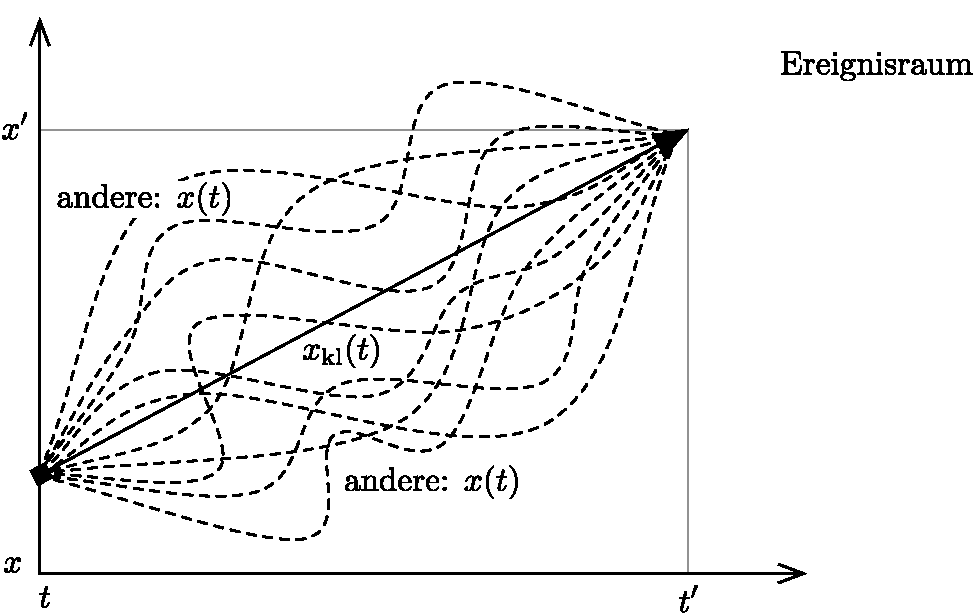
\includegraphics[scale=.75]{Figs/Pfade}
\end{figure}\vspace{-4ex}

Die Pfadintegralformulierung und ihr Bezug zur bereits wohl bekannten Formulierung der Quantenmechanik lässt sich  besser Verstehen, wenn wir uns das {\bf Doppelspaltexperiment} noch einmal vergegenwärtigen. Dort ist die Wahrscheinlichkeit das Teilchen im Abstand $d_i$ vom Spalt $i\in\{1,2\}$ zu finden durch das Betragsquadrat von $\psi_i\propto\e^{\I\;k\,d_i}$ gegeben, sofern nur ein Spalt offen ist und sofern beide Spalte offen sind durch das Betragsquadrat von $\psi_1+\psi_2$. Dass sich die Wahrscheinlichkeiten auf diese eigenartige Weise aufsummieren, ist dabei eine experimentelle Beobachtung. Wir können uns nun das Experiment verallgemeinert vorstellen für unendlich viele Spalte. Die Wahrscheinlichkeitsamplitude ist dann durch das Integral über die Einzelamplituden gegeben. Die Form der Einzelamplituden können wir uns erschließen, wenn wir uns an die Herleitung der Wellenmechanik in Analogie zur Eikonalgleichung erinnern, in der die Amplituden gegeben sind durch Wellen konstanter Wirkung $\psi=\e^{\;\I/\hbar\cdot S_0}$, so dass für $\hbar\to0$ die Schrödingergleichung in die Hamilton-Jacobi-Gleichung übergeht. Damit sind wir bis auf den Vorfaktor wieder bei der Definition des Propagators. 

Es wird nun auch der Übergang zur klassischen Mechanik leichter deutlich, welche sich also für $S/\hbar\to\infty$ ergeben sollte. Dies lässt sich dadurch erklären, dass in diesem Fall der Phasenfaktor stark oszilliert und somit im Mittel nicht zum Integral beiträgt. Nur der klassische Pfad $x_{\text{kl}}$, für den nach dem Hamiltonschen Prinzip die Wirkung ja stationär $\delta S=0$ wird trägt dann noch zur Zeitentwicklung bei. 

Es ist außerdem anzumerken, dass die Pfadintegralformulierung insbesondere zwei wichtige Vorteile in der Anwendung hat: 
\begin{itemize1}
	\item Zum einen bietet sich die Pfadintegralformulierung durch die Formulierung mittels Integralen für numerische Berechnungen an und lässt sich einfacher approximieren. 
	\item Zum anderen vereinfacht sie die Quantisierung von {\bf Eichtheorien}, da im Gegensatz zur Operatorformulierung die Zeitvariable nicht besonders behandelt werden muss, was in relativistischen Formulierungen, in denen Kovarianz erfüllt sein muss, gewisse Schwierigkeiten hervorruft, die im Pfadintegralformalismus hingegen nicht auftreten. Mehr dazu im nächsten Abschnitt. 
\end{itemize1}


\paragraph{Tunneln aus metastabilem Zustand}

Wir wollen im folgenden als Beispielhafte Anwendung des Pfadintegralformalismus einen eindimensionalen Tunnelprozess in $x$-Richtung zwischen den Punkten $0$ und $a$ im Potential $V(x)$ betrachten. Der klassische Pfad stationärer Wirkung der Lagrangefunktion $\mathcal{L}=T(\dot{x})-V(x)=m/2\cdot\dot{x}^2-V(x)$ kann in diesem Fall für imaginäre Zeiten: $t\to \I\tau$ einfach bestimmt werden. Die Bewegungsgleichung $\mathrm{d}/\mathrm{d}t\;\dell_{\dot{x}}\,\mathcal{L}=-\dell_x\,\mathcal{L}$ kann dann in Abhängigkeit von $\tau$ geschrieben werden als: 
\begin{eqnarray*}
	m\cdot\dell_t^2\; x = -\dell_x\; V(x) &\quad\overset{t\to \I\tau}{\Rightarrow}\quad& m\cdot \dell_{\tau}^2\; x = \dell_x\; V(x) 
\end{eqnarray*}
Dies entspricht der Bewegung im Potential mit umgedrehten Vorzeichen $V(x)\to-V(x)$, also $\mathcal{L}=T(\dell_{\tau}x)+V(x)$. Da in dem System Energieerhaltung $\dell_{\tau} \ham = 0$ gilt, können wir ohne Beschränkung der Allgemeinheit $\ham=T-V=E=:0$ setzen, so dass sich $m/2\cdot(\mathrm{d}x/\mathrm{d}\tau)^2 = V(x)$ ergibt. Damit folgt für die Wirkung entlang des klassischen Pfads $S\big(x_{\text{kl}}(t),0,\tau\big)$: 
\begin{eqnarray*}
	-\I\cdot S\big(x_{\text{kl}},0,t\big) &=& \int_0^{\tau}\mathrm{d}\tau'\!\!\!\!\!\!\!\!\!\!\!\!\!\!\!\!\!\!\!\!\!\!\!\!\!\underbrace{\frac{m}{2}\cdot\Big(\frac{\mathrm{d}x}{\mathrm{d}\tau}\Big)^2+V(x)}_{\qquad\quad\qquad=\;m(\mathrm{d}x/\mathrm{d}\tau)^2\;=\;m\;\mathrm{d}x/\mathrm{d}\tau\cdot\sqrt{2V(x)/m}}\!\!\!\!\!\!\!\!\!\!\!\!\!\!\!\!\!\!\!\!\!\!\!\!\! = \int_0^{\tau} \mathrm{d}\tau'\;\frac{\mathrm{d}x}{\mathrm{d}\tau'}\; \sqrt{2mV(x)} = \int_0^a\mathrm{d}x\; \sqrt{2m V(x)}
\end{eqnarray*}
Der führende Ausdruck im Propagator ist damit der Näherungsausdruck für die Tunnelamplitude, wie er sich aus der Wentzel–Kramers–Brillouin ({\bf WKB}) Methode ergibt: 
\begin{eqnarray*}
	K(0,0,a,t) &\approx& C\cdot\e^{\;\frac{\I}{\hbar}\cdot S(x_{\text{kl}},0,t)}=C\cdot\e^{\;\frac{1}{\hbar}\cdot\int_0^a\mathrm{d}x\;\sqrt{2mV(x)}}
\end{eqnarray*}


\paragraph{Statistische Mechanik eines Teilchens}
Die Zustandsumme $Z$ eines Teilchens im Potential $V(x)$ ist in der statistischen Mechanik gegeben durch: 
\begin{eqnarray*}
	Z &=& \Sp\big(\e^{-\beta\hat{\ham}}\,\big) = \int \mathrm{d}x\; \bracket{x}{\e^{-\beta\hat{\ham}}}{x} \qquad \text{mit: } \beta=\frac{1}{k_BT}
\end{eqnarray*}
Sie spielt eine wichtige Rolle, da sie in der Maxwell-Boltzmann-Verteilung auftaucht, welche die Wahrscheinlichkeit $p_{E_n}$ beschreibt, das das System in einem bestimmten Zustand der Energie $E_n$ zu finden: $p_{E_n}=1/Z\cdot\e^{-\beta E_n}$. 

Wir sehen, dass die Zustandssumme dabei grade dem Propagator $K(x,0,x,t)=\bracket{x}{\e^{-\I/\hbar\cdot \hat{\ham}t}}{x}$ entspricht, wenn wir die imaginäre Zeit $t\to \I\hbar \beta$ verwenden. Es ergbit sich dann folgender Ausdruck für die Zustandssumme als Pfadintegral: 
\begin{eqnarray*}
	Z \;= \int\mathrm{d}x\;\bracket{x}{\e^{-\beta\hat{\ham}}}{x} \;= \int \mathrm{d}x\!\!\!\!\underset{x(0)=x,\;x(\beta)=x}{\int \mathscr{D}x} \e^{-\frac{1}{\hbar}\int_0^{\hbar\beta}\mathrm{d}\tau\; \frac{m}{2}\left(\!\frac{\mathrm{d}x}{\mathrm{d}\tau}\!\right)^2+V(x)}
\end{eqnarray*}
Das Pfadintegral berücksichtigt dabei die quantenmechanischen Fluktuationen, welche proportional zu $\Delta x$  sind. Es gilt: 
\begin{eqnarray*}
	\Delta x \propto \sqrt{\frac{2\pi \hbar^2}{m k_B T}} =: \lambda_{\text{therm}}
\end{eqnarray*}
Wobei $\lambda_{\text{therm}}$ als thermodynamische De-Broglie-Wellenlänge bezeichnet wird. Im klassischen Grenzfall, wenn sich $V(x)$ auf der Scala von $\lambda_{\text{therm}}$ nur wenig ändert, können wir den Propagator dann auf den Propagator eines freien Teilchens $K_{\text{frei}}$ reduzieren und es ergibt sich die klassische Zustandssumme mit dem bekannten Vorfaktor: 
\begin{eqnarray*}
	Z \;= \int\mathrm{d}x\;\bracket{x}{\e^{-\beta\hat{\ham}}}{x} \;\approx\; \int \mathrm{d}x\;\e^{-\beta V(x)}\cdot\!\!\!\!\!\!\!\!\! \underbrace{\underset{x(0)=x,\;x(\beta)=x}{\int \mathscr{D}x} \e^{-\frac{m}{2\hbar}\int_0^{\hbar\beta}\mathrm{d}\tau\; \left(\!\frac{\mathrm{d}x}{\mathrm{d}\tau}\!\right)^2}}_{=\; K_{\text{frei}}(x,-\I\hbar\beta,x,0)\;=\;\sqrt{\frac{mk_BT}{2\pi\hbar^2}}} &=& \int \mathrm{d}x\;\;\frac{\e^{-\beta V(x)}}{\lambda_{\text{therm}}}
\end{eqnarray*}




\subsubsection{Eichtransformationen in der Quantenmechanik}

Als Eichtransformation bezeichnet man eine Transformation sogenannter Eichfelder, beispielsweise die elektromagnetischen Potentiale, unter der die Dynamik eines Systems invariant bleibt. Man unterscheidet dabei zwischen {\bf globalen Eichtransformationen}, welche die Eichfelder an allen Orten um einen Faktor verschiebt, Beispiel hierfür sind Nullpunktsverschiebungen, und {\bf lokalen Eichtransformationen}, welche die Eichfelder um eine ortsabhängige Funktion verschiebt. Wenn die Dynamik einer Feldtheorie aus einer lokal eichinvarianten, also unter Eichtransformationen unveränderten, Wirkung folgt, so wird die physikalsiche Theorie auch als {\bf Eichtheorie} bezeichnet und man spricht davon, dass die Theorie einer lokalen Eichsymmetrie genügt. 

Wir haben gesehen, dass sich die Quantenmechanik durch den Pfadintegralformalismus aus der Wirkung ableiten lässt und wir erinnern uns, dass die Wirkung für elektromagnetische Felder im klassischen Fall eichinvariant war. Die Quantenmechanik sollte also auch eine Eichtheorie sein. Dies wollen wir im folgenden auch explizit in der kanonischen Formulierung der Quantenmechanik zeigen. 

Dazu erinnern wir uns zunächst, dass der Hamiltonoperator $\hat{\ham}$ eines Teilchens in einem elektromagnetischen Feld mit skalarem Potential $\hat{\phi}(\hat{\vec{r}},t)$ und Vektorpotential $\hat{\vec{A}}(\hat{\vec{r}},t)$ gegeben war durch:
\begin{eqnarray*}
	\hat{\ham}(\hat{\vec{r}},\hat{\vec{p}},t) &=& \frac{1}{2m}\cdot \big(\hat{\vec{p}}-q\cdot\hat{\vec{A}}(\hat{\vec{r}},t)\big)^2 + q\cdot\hat{\phi}(\hat{\vec{r}},t)
\end{eqnarray*}
Wir definieren nun den {\bf Geschwindigkeitsoperator} $\hat{\vec{v}}=\mathrm{d}/\mathrm{d}t\;\hat{\vec{r}}$, dessen explizite Darstellung sich aus der Heisenberg Gleichung (\ref{HG}) ergibt zu: 
\begin{eqnarray*}
	\hat{\vec{v}} &=& \frac{\mathrm{d}}{\mathrm{d}t}\;\hat{\vec{r}} = - \frac{\I}{\hbar} [\hat{\vec{r}},\hat{\ham}] = -\frac{\I}{2m\hbar}\Big[\hat{\vec{r}}\;,\;\hat{\vec{p}}\,^2-q\cdot\hat{\vec{p}}\hat{\vec{A}}- q\cdot\hat{\vec{A}}\hat{\vec{p}}\,\Big] = -\frac{1}{m}\cdot(\hat{\vec{p}}-q\cdot \hat{\vec{A}}\,)
\end{eqnarray*} 
Dabei vertauschen die Komponenten des Geschwindigkeitsoperators $\hat{v}_i$ mit $i\in\{x,y,z\}$ nicht untereinander und es lässt sich mit Hilfe von $\hat{\vec{B}}=\rot\hat{\vec{A}}$ folgende Relation finden: 
\begin{eqnarray*}
	[\hat{v}_i,\hat{v}_j] &=& -\frac{q}{m^2}\cdot \underset{\;}{\Big(} [\hat{p}_i,\hat{A}_j] + [\hat{A}_i,\hat{p}_j] \Big) = \frac{\I\hbar q}{m^2}\cdot(\partial_i\hat{A}_j-\partial_j\hat{A}_i) = \frac{\I\hbar q}{m^2}\cdot \varepsilon_{ijk}\hat{B}_k
	\\
	&&\Rightarrow\quad \hat{\vec{v}}\times\hat{\vec{v}} = \frac{\I q\hbar}{m^2}\cdot \hat{\vec{B}}
\end{eqnarray*} 
Mit Hilfe des Geschwindigkeitsoperators $\hat{\vec{v}}(\hat{\vec{r}},\hat{\vec{p}},t)$ können wir den Hamiltonoperator $\hat{\ham}$ nun schreiben wie folgt:
\begin{eqnarray*}
	\hat{\ham}(\hat{\vec{r}},\hat{\vec{p}},t) &=& \frac{m}2\cdot\hat{\vec{v}}(\hat{\vec{r}},\hat{\vec{p}},t)^2 + q\cdot\hat{\phi}(\hat{\vec{r}},t) 
\end{eqnarray*}
Die {\bf Wahrscheinlichkeitsstromdichte} $\vec{j}$ ergibt sich nun mit dem verallgemeinerten Impulsoperator im Ortsraum $\hat{\vec{p}}\to m\cdot\hat{\vec{v}}=-\I\hbar\cdot\vec{\nabla}-q\cdot\vec{A}$ zu: 
\begin{eqnarray*}
	\vec{j} &=& \frac{1}{2m} \cdot\Big(\psi^*(-\I\hbar\cdot\vec{\nabla}-q\cdot\vec{A}\,)\;\psi - \psi\;(-\I\hbar\cdot\vec{\nabla}-q\cdot\vec{A}\,)\;\psi^*\underset{\;}{\Big)}
	\\
	&=& -\frac{\I\hbar}{2 m}\cdot\big(\psi^*(\vec{\nabla}\psi)-\psi\;(\vec{\nabla}\psi^*)\big) - \frac{q}{m} \cdot |\psi|^2 \vec{A}
\end{eqnarray*}
Und erfüllt wie man leicht sieht weiterhin die Kontinuitätsgleichung: $\partial_t |\psi|^2+\vec{\nabla}\vec{j}=0$.

Wir wollen nun das Verhalten unter den folgenden aus der Elektrodynamik bekannten lokalen Eichtransformationen im Ortsraum an den Potentialen betrachten, welche zwar den Hamiltonoperator verändern werden, die elektromagnetischen $\vec{E}$- und $\vec{B}$-Felder jedoch unverändert lässt:
\begin{alignat*}{4}
	\vec{A}(\vec{r},t) &\qquad\to\qquad& \vec{A}\,'(\vec{r},t) &\;=\;\;& \vec{A}(\vec{r},t) + \vec{\nabla}\Lambda(\vec{r},t)
	\\
	\phi(\vec{r},t) &\qquad\to\qquad& \phi'(\vec{r},t) &\;=\;\;& \phi(\vec{r},t) - \dell_t\Lambda(\vec{r},t)
\end{alignat*}
Wir wollen nun zeigen, dass sich die Eichinavrianz der Schrödingergleichung unter dieser Eichtransformation durch eine lokale Phasentransformation der Wellenfunktion $\psi(\vec{r},t)$ mit dem unitären Operator $U(\vec{r},t)$ erreichen lässt: 
\begin{alignat*}{4}
	\psi(\vec{r},t) &\qquad\to\qquad& \psi'(\vec r,t) &\;=\;\;& \underbrace{\e^{\;\frac{\I}{\hbar}q\cdot \Lambda(\vec{r},t)}}_{=\;U(\vec{r},t)} \psi(\vec{r},t) = U(\vec{r},t)\cdot\psi(\vec{r},t)
\end{alignat*}
Wir wollen nun die Wirkung der Eichtransformation auf die Operatoren $\hat{\vec{r}}$, $\hat{\vec{p}}$ und $\hat{\vec{v}}$ untersuchen. Dazu untersuchen wir die Erwartungswerte der Operatoren $\hat{\vec{o}}\,$: 
\begin{eqnarray*}
	\EW{\hat{\vec{o}}\,}'=\bracket{\psi'}{\hat{\vec{o}}\,}{\psi'}=\bracket{\psi}{\hat{U}^{\dagger}\hat{\vec{o}}\,\hat{U}}{\psi}=\EW{\hat{U}^{\dagger}\hat{\vec{o}}\,\hat{U}} &\quad\Rightarrow\quad& \EW{\hat{\vec{o}}\,}'=\EW{\hat{\vec{o}}\,}\;\Leftrightarrow\;[\hat{\vec{o}},\hat{U}]=0
\end{eqnarray*}
Ein Operator ist also invariant unter der Eichtransformation wenn er mit dem unitären Operator $\hat{U}$ der Phasentransformation vertauscht. Für die Operatoren $\hat{\vec{r}}$ und $\hat{\vec{p}}$ ergibt sich somit bei der Untersuchung im Ortsraum folgendes: 
\begin{eqnarray*}
	\big[\vec{r},U(\vec{r},t)\big] &=& 0  
	\\
	\big[\hat{\vec{p}},U(\vec{r},t)\big] &=& \big[-\I\hbar\cdot\vec{\nabla},U(\vec{r},t)\big] = -\I\hbar\cdot\big(\vec{\nabla}U(\vec{r},t)\big) = q\cdot\big(\vec{\nabla}\Lambda(\vec{r},t)\big)\cdot U(\vec{r},t) \neq 0
\end{eqnarray*}
Der Impulsoperator ist also nicht eichinvariant, der Ortsoperator hingegen schon. Wir wollen nun noch den Geschwindigkeitsoperator $\hat{\vec{v}}$ betrachten, für den wir folgende Beziehung finden können: 
\begin{eqnarray*}
	m\cdot U^{\dagger}\hat{\vec{v}}\,U &=& U^{\dagger}(\hat{\vec{p}}-q\cdot\vec{A}\,)U = U^{\dagger}(U\hat{\vec{p}}+\!\!\!\!\!\!\!\underbrace{[\,\hat{\vec{p}},U]}_{\quad=\;q\cdot U (\vec{\nabla}\Lambda)}\!\!\!\!\!\!)-q\cdot U^{\dagger}U\vec{A} = \hat{\vec{p}} -q\cdot(\vec{\nabla}\Lambda+\vec{A}) 
	\\
	&=& \hat{\vec{p}}-q\cdot\vec{A}\,'= m\cdot\hat{\vec{v}}\,' \qquad\qquad\qquad\qquad\qquad\qquad\Rightarrow\quad\EW{\hat{\vec{v}}\,}=\EW{\hat{\vec{v}}\,'}'
\end{eqnarray*}
Die Schrödingergleichung $\I\hbar\cdot\dell_t \psi=\hat{\ham}\psi$ ist somit invariant, wenn wir den Hamiltonoperator transformieren $\hat{\ham}\to\hat{\ham}'$ zu:
\begin{eqnarray*}
	\hat{\ham}' &=& U\hat{\ham}U^{\dagger}+\I\hbar\cdot U^{\dagger}\partial_t U = \frac{m}{2}\cdot \hat{\vec{v}}\,'\,\!^2+q\cdot\hat{\phi}-q\cdot\dell_t\Lambda = \frac{m}{2}\cdot \hat{\vec{v}}\,'\,\!^2+q\cdot\hat{\phi}' \quad\Rightarrow\quad \I\hbar\dell_t\psi'=\hat{\ham}'\psi'
\end{eqnarray*}
Wir können somit als Fazit festhalten, dass die Quantenmechanik tatsächlich invariant ist unter den aus der Elektrodynamik bekannten Eichtransformationen und sich die Zustände um einen Phasenfaktor transformieren $\psi' =\psi\cdot\e^{\;\I/\hbar\cdot q\Lambda(\vec{r},t)}$, welcher keinen Einfluss auf die physikalischen Ergebnisse hat. 


\subsubsection{Der Aharonov-Bohm-Effekt}

Wir wollen uns im folgenden noch mit einem interessanten Effekt Beschäftigen, welcher aus der Struktur der quantenmechanischen Theorie folgt und ein neues Licht auf die Bedeutung der Potentiale von Feldern wirft, welche in der klassischen Mechanik ja keine physikalische Existenz haben, sondern nur mathematische Hilfskonstrukte sind. 

Dazu stellen wir uns ein Doppelspaltexperiment vor und fügen zwischen den beiden Spalten eine Box ein, in der ein Magnetfeld $\vec{B}$ herrscht welches allerdings vom Außenraum komplett abgeschirmt ist: $\vec{B}(\vec{r}\notin\text{Box}) = 0$. Das Vektorpotential $\vec{A}$ erstrecke sich jedoch auf den gesamten Raum. Die folgende Abbildung soll diesen Aufbau veranschaulichen: 
\vspace{-2ex}\begin{figure}[!h]\centering
	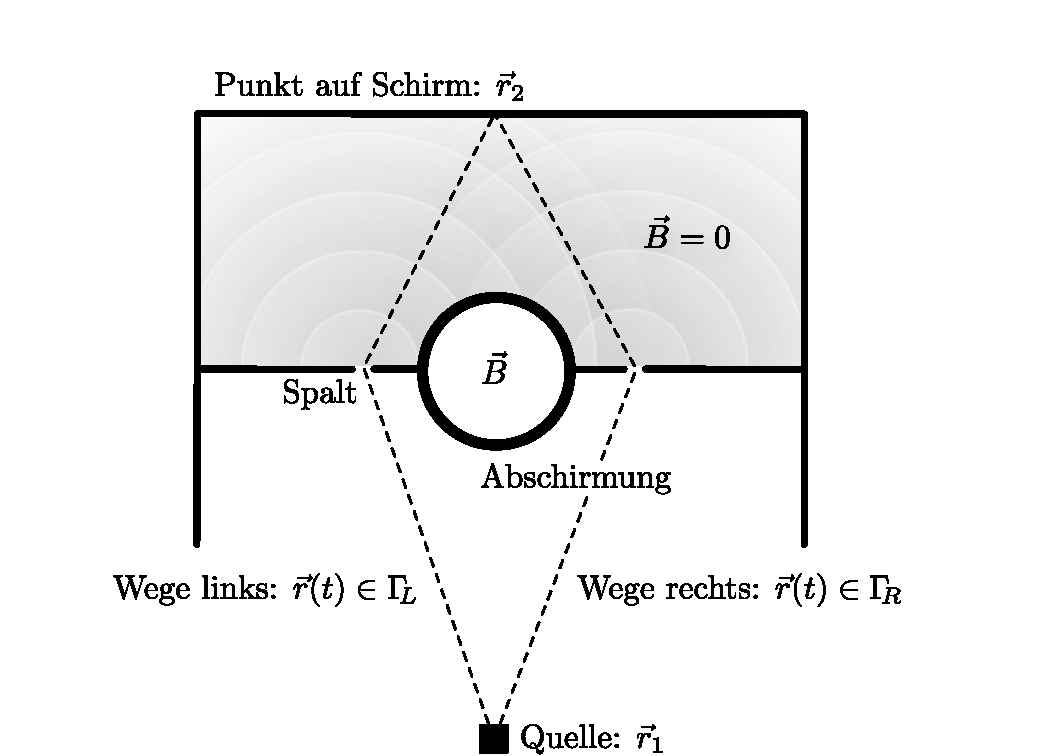
\includegraphics[scale=0.75]{Figs/DoppelspaltB}
\end{figure}

Wir wollen nun untersuchen, ob die Präsenz des Feldes $\vec{B}=\rot\vec{A}$ einen Einfluss auf unsere Messung hat. Dazu definieren wir zunächst den magnetischen Fluss $\phi_B(A)$ durch eine Fläche $A$, welcher nach dem Satz von Stokes für ein Magnetfeld durch die Fläche $A$ mit Normalenvektor $\vec{n}_A$ und Rand $\dell A$ gegeben ist durch:
\begin{eqnarray*}
	\phi_B(A) &=& \int_A\mathrm{d}\vec{A}\;\vec{B} = \int_A\mathrm{d}\vec{n}_A\; \vec{\nabla}\times\vec{A} = \oint_{\dell A}\mathrm{d}\vec{s}\; \vec{A} 
\end{eqnarray*}
Um die Bedingung zu erfüllen, dass das $\vec{B}$-Feld im Außenraum verschwindet, können wir das Vektorpotential $\vec{A}$ beispielsweise als reines Gradientenfeld definieren: $\vec{A}(\vec{r})=\vec{\nabla}\Lambda(\vec{r})$. Wenn wir beispielsweise ein Magnetfeld $\vec{B}$ betrachten, welches einen Zylinder mit Radius $R$ in $z$-Richtung durchdringt, so ergibt sich der gesamte magnetische Fluss durch die Fläche $\pi R^2$ zu $\phi_B=\pi R^2\cdot B$. Ein mögliches $\Lambda$ um das zugehörige Vektorpotential $\vec{A}$ als Gradientenfeld zu definieren wäre dann in Zylinderkoordinaten $\vec{r}=\varphi\cdot\vec{e}_{\varphi}+\rho\cdot\vec{e}_{\rho}+z\cdot\vec{e}_{z}$ beispielsweise durch $\Lambda=\phi_B/1\pi\cdot\varphi$ gegeben. Das Vektorpotential ergibt sich dann zu $\vec{A}=\phi_B/2\pi\rho\cdot \vec{e}_{\varphi}$. Die mögliche Wahl des Vektorpotentials als reines Gradientenfeld und nicht einfach als 0 ist dabei eine direkte Folge der Eichinvarianz, wegen der das verschwindende magnetische Feld $\vec{B}=0$ das Vektorpotential eben nicht eindeutig, sondern nur bis auf eine Eichtransformation bestimmt. 

Wir wollen nun betrachten, was mit dem Interferenzbild passiert. Dabei lässt sich aus den Überlegungen im vorigen Abschnitt einsehen, dass sich durch die Eichtransformation ein Phasenfaktor ergibt, der potentiell Einfluss auf die Wahrscheinlichkeitsamplitude haben kann, da sich diese ja als Betragsquadrat aus der Summe der Wellenfunktion für den Weg durch beide Spalte ergibt. Wenn zwischen den beiden Wegen also durch das Einschalten des Potentials ein Phasenunterschied vorliegt, so verändert sich das Interferenzmuster. Wir wollen dies im folgenden anhand des Propagators näher untersuchen. 

Wenn wir einen Propagator von der Quelle am Ort $\vec{r}_1=\vec{r}(t_1)$ zu einem Punkt auf dem Schirm bei $\vec{r}_2=\vec{r}(t_2)$ betrachte, so ergibt sich der Propagator zu:
\begin{eqnarray*}
	K(\vec{r}_1,t_1,\vec{r}_2,t_2) &=& \!\!\!\!\!\!\!\!\!\!\!\underset{\vec{r}(t_2)=\vec{r}_2,\;\vec{r}(t_1)=\vec{r}_1}{\int\mathscr{D}\vec{r}} \!\!\!\! \e^{\;\frac{\I}{\hbar} S(\vec{r}(t),t_1,t_2)} 
\end{eqnarray*}
Die Wirkung ergibt sich dabei für ein Teilchen im Vektorpotential $\vec{A}$ zu: 
\begin{eqnarray*}
	S\big(\vec{r}(t),t_1,t_2\big) = \underbrace{\int_{t_1}^{t_2}\!\!\!\!\mathrm{d}t\; \Big(\frac{m}{2}\cdot \dot{\vec{r}}\,^2 - V(\vec{r})\Big)}_{=\;S(\vec{r}(t),t_1,t_2)\left|_{\vec{A}=0}\right.} + \;q\cdot\!\!\!\!\!\!\!\!\!\!\!\!\!\underbrace{\int_{t_1}^{t_2}\!\!\!\!\mathrm{d}t\;\dot{\vec{r}}\vec{A}}_{\qquad =\;\int_{\gamma(\vec{r}_1,\vec{r}_2)}\mathrm{d}\vec{s}\;\vec{A}}\!\!\!\!\!\!\!\!\! = S\big(\vec{r}(t),t_1,t_2\big)\big|_{\vec{A}=0}+q\cdot\!\!\underbrace{\big(\Lambda(\vec{r}_2)-\Lambda(\vec{r}1)\big)}_{=\;\phi_B(\vec{r}(t),\vec{r}_1,\vec{r}_2)}
\end{eqnarray*}
Dabei ist $\phi_B\big(\vec{r}(t),\vec{r}_1,\vec{r}_2\big)$ magnetische Fluss durch die vom Weg $\vec{r}(t)$ zwischen $\vec{r}_1$ und $\vec{r}_2$ eingeschlossene Fläche. Wir wollen nun die Gesamtheit der Wege aufteilen in die Menge aller Wege durch den linken Spalt $\Gamma_{\!\!L}$ und die Menge aller Wege durch den rechten Spalt $\Gamma_{\!\!R}$. Dabei unterscheidet sich die Wirkung in diesen beiden Teilmengen strukturell nicht im Teil $S\big(\vec{r}(t),t_1,t_2\big)\big|_{\vec{A}=0}$. Wir können dann das Pfadintegral aufteilen in zwei Teile und folgendes schreiben: 
\begin{eqnarray*}
	&&K(\vec{r}_1,t_1,\vec{r}_2,t_2) \quad=\quad \int_{\vec{r}_1}^{\vec{r}_2}\!\!\!\!\!\mathscr{D}\vec{r}\; \e^{\;\frac{\I}{\hbar} S(\vec{r}(t),t_1,t_2)} \;\Big|_{\vec{r}(t)\,\in\,\Gamma_{\!L}} \!\!\!+ \int_{\vec{r}_1}^{\vec{r}_2}\!\!\!\!\!\mathscr{D}\vec{r}\; \e^{\;\frac{\I}{\hbar} S(\vec{r}(t),t_1,t_2)} \;\Big|_{\vec{r}(t)\,\in\,\Gamma_{\!R}} 
	\\
	&&\quad = \int_{\vec{r}_1}^{\vec{r}_2}\!\!\!\!\!\mathscr{D}\vec{r}\; \e^{\;\frac{\I}{\hbar} \left(S(\vec{r}(t),t_1,t_2)\left|_{\vec{A}=0}\right.+q\phi_B(\vec{r}(t),\vec{r}_1,\vec{r}_2)\right)} \;\Big|_{\vec{r}(t)\,\in\,\Gamma_{\!L}} \!\!\!+ \int_{\vec{r}_1}^{\vec{r}_2}\!\!\!\!\!\mathscr{D}\vec{r}\; \e^{\;\frac{\I}{\hbar} \left(S(\vec{r}(t),t_1,t_2)\left|_{\vec{A}=0}\right.+q\phi_B(\vec{r}(t),\vec{r}_1,\vec{r}_2)\right)} \;\Big|_{\vec{r}(t)\,\in\,\Gamma_{\!R}}
	\\
	&&\quad = \int_{\vec{r}_1}^{\vec{r}_2}\!\!\!\!\!\mathscr{D}\vec{r}\; \e^{\;\frac{\I}{\hbar} S(\vec{r}(t),t_1,t_2)\left|_{\vec{A}=0}\right.} \cdot \underbrace{\e^{\;\frac{\I}{\hbar}q\cdot\left(\phi_B(\vec{r}(t),\vec{r}_1,\vec{r}_2)\left|_{\vec{r}(t)\in\,\Gamma_{\!L}}\right.-\phi_B(\vec{r}(t),\vec{r}_2,\vec{r}_1)\left|_{\vec{r}(t)\in\,\Gamma_{\!R}}\right.\right)}}_{=:\;\e^{\I/\hbar\cdot q\cdot\Delta_{LR}\,\phi_{B}}}
\end{eqnarray*}
Der Phasenunterschied zwischen den Wegen auf der rechten Seite $\gamma\in\Gamma_{\!\!R}$ und der linken Seite $\gamma\in\Gamma_{\!\!L}$ ergibt sich dabei zu: 
\begin{eqnarray*}
	\quad\Delta_{LR}\,\phi_{B} = \frac{q}{\hbar}\cdot \bigg(\int_{\gamma(\vec{r}_1,\vec{r}_2)\in\Gamma_{\!L}}\!\!\!\!\!\!\!\!\!\!\!\!\!\!\!\!\!\!\mathrm{d}\vec{s}\;\vec{A}\;\;-\int_{\gamma(\vec{r}_2,\vec{r}_1)\in\Gamma_{\!R}}\!\!\!\!\!\!\!\!\!\!\!\!\!\!\!\!\!\!\mathrm{d}\vec{s}\;\vec{A}\quad\bigg) = \frac{q}{\hbar}\oint_{\gamma\in\,\Gamma_{\!L}\times\Gamma_{\!R}}\!\!\!\!\!\!\!\!\!\!\!\!\!\!\!\mathrm{d}\vec{s}\; \vec{A} = 2\pi\cdot\!\!\!\!\!\underbrace{\frac{q}{2\pi\hbar}}_{\quad=\;1/\Phi_0}\!\!\!\!\! \cdot\phi_B(A_{\gamma}) = 2\pi\cdot\frac{\phi_B(A_{\gamma})}{\Phi_0} 
\end{eqnarray*}
Dabei wird $\Phi_0$ als Flussquantum bezeichnet. Wir sehen also, dass die Phase nur davon abhängt, ob die möglichen Wege den Fluss eines magnetischen Feldes durch eine Fläche einschließen, nicht ob sie durch diesen führen. Und wir sehen, dass die Postition der Interferenzmaxima durch die Existenz dieses magnetischen Flusses abhängt, weil sie den Propagator signifikant beeinflusst. 

Wir können also festhalten, dass in der Quantenmechanik nicht nur Kraftfelder Einfluss auf die Dynamik eines Systems nehmen können, sondern auch ohne den direkten Einfluss eines Lorentzkraft auf ein geladenenes Teilchen, dessen Bewegung beeinflusst werden kann. Dies ist direkt dadurch bedingt, dass in der Quantenmechanik die Dynamik nicht furch einen determinierten Weg des Teilchens beschrieben wird, sondern alle möglichen Wege die Dynamik des Teilchens beeinflussen und somit ein durch diese Möglichen Wege eingeschlossener Fluss einen Einfluss haben kann. 

Die Interpretation der Kraftfelder stellt einen bedeutenden Unterschied der Quantenmechanik zur klassischen Mechanik da. Es gibt generell zwei Möglichkeiten die Bedeutung von Feldern in der Quantenmechanik zu interpretieren: 
\begin{itemize1}
\item Entweder in der Quantenmechanik sind die elektromagnetischen Potentiale $\vec{A}$ und $\phi$ die Grundlegenden physikalische Größen, anstelle der Felder $\vec{E}$ und $\vec{B}$. Jedoch gilt für sie weiterhin die Eichfreiheit. 
\item Oder die Felder $\vec{E}$ und $\vec{B}$ werden weiterhin als die Grundlegenden physikalische Größen betrachtet, aber es wird akzeptiert, dass sie auf nicht-lokale Weise wechselwirken können. Es müsste also die {\bf Lokalität} der Theorie aufgegeben werden. 
\end{itemize1}

%\end{document}